\chapter{Shape-Change Termination}

Size-change termination, despite being simple is powerful enough to determine
the halting property for a large class of programs. Many authors have extended
the principle to even wider classes of programs, e.g. extending it to handle
initially not well-founded data types \cite{bound-analysis}, applying it in
imperative programming languages \cite{heaps}, etc. 

One trouble with size-change termination as described in the previous chapter
is \referToLemma{cycle-reduce}. This lemma makes size-change termination weak
in the sense that the overall shape changes in a given call cycle are
\emph{not} considered, and instead, call cycles are constrained to
monotonically decreasing call cycles.  However, there may be programs that have
calls, or even call cycles, that in terms of size, increase a value for a
finite amount of time, until some condition is met, or as in the case of \D{},
a value has some particular shape.

Consider the program in \referToListing{size-change-fail} as an example of a
program for which regular size-change termination is unable to determine the
halting property, while the property itself would seem fairly simple to deduce.
This is a sample program where some value is increased in terms of size in a
call cycle, but only until the value matches a certain shape, the shape
required by a terminal clause.

\begin{lstlisting}[
  label=listing:size-change-fail,
  caption={A terminating program with a call cycle where a value is
  temporarily increased.}]
$f_0$: f a.b.c.d := a
$f_1$: f a := f a.0
f input
\end{lstlisting}

The extension proposed in this chapter is to be able to determine the halting
property for such a class of programs without reducing size of the class of
programs for which size-change termination can already deduce the halting
property.

In the discussion below we continue the assumptions from
\referToSection{size-change-termination}. In particular, all clauses in a
program are unary and bind at most one variable. Also, we can safely disregard
terminal clauses in call graphs.

\section{The class of programs considered}

Before we can speak of extending size-change termination to determine the
halting property for programs in the same class as
\referToListing{size-change-fail}, we need to formally define that class.

Actual conditions in \D{} can only be expressed in terms of patterns in
function clauses. Hence, we disregard programs that rely on equality or size
comparison conditions for termination, since this type of programs will often
already be covered by regular size-change termination, and if not, they at the
very least come down to recursive pattern matching.

As an example of a program where size-change termination is already prevalent,
consider a program that finds the $n^{th}$ Fibonacci number as the one already
presented in \referToSection{d-samples}. The function \mono{fibonacci-aux}
seemingly increases a value until a condition is met, in particular, until we
count one of the arguments down to \mono{0}. However, due to the fact that we
count that we decrease the value of that argument in \emph{recursive} clause of
the \mono{fibonacci-aux} functions, the halting property is certainly already
deducible by regular size-change termination.

Instead, we turn our attention to simpler programs, ones that rely solely on
conditions defined in terms of patterns. Consider again the program in
\referToListing{size-change-fail}. The function \mono{f} has only one terminal
clause, the one that accepts a shape as in \referToFigure{size-change-fail-f0}.
If the function argument has any other shape, i.e. either a shape as in
\referToFigure{size-change-fail-f1-0}, \referToFigure{size-change-fail-f1-1} or
\referToFigure{size-change-fail-f1-2}, then the recursive clause $f_1$ is
chosen. For any argument $b\in\mathbb{B}$, the clause $f_1$ replaces the
right-most child of the value, which is always \mono{0}, with a node.

For instance, the smallest possible argument $b\in\mathbb{B}$ is \mono{0}.  If
passed such a value, $f_1$ transforms it into a value that has a shape that
corresponds to \referToFigure{size-change-fail-f1-1}, which in turn transforms
the value into one that matches \referToFigure{size-change-fail-f1-2}, which in
turn transforms the value into one that matches
\referToFigure{size-change-fail-f0}, i.e. the terminal clause. What's more,
there are infinitely many other values that will match the shape
\referToFigure{size-change-fail-f1-1}, and for each of them, the clause $f_1$
will transform them into values that match
\referToFigure{size-change-fail-f1-2}, which will transform them into values
that match \referToFigure{size-change-fail-f0}.

\includeFigure{size-change-fail-f0}{The shape that the clause $f_0$ in
\referToListing{size-change-fail} will accept.}

\begin{figure}[htbp!]
\begin{minipage}{0.3\linewidth}
\centering
\includegraphics{figures/size-change-fail-f1-0}
\caption[]{The pattern \mono{0}.}
\label{figure:size-change-fail-f1-0}
\end{minipage}
\begin{minipage}{0.3\linewidth}
\centering
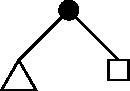
\includegraphics{figures/size-change-fail-f1-1}
\caption[]{The pattern \mono{a.0}.}
\label{figure:size-change-fail-f1-1}
\end{minipage}
\begin{minipage}{0.3\linewidth}
\centering
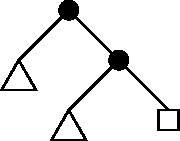
\includegraphics{figures/size-change-fail-f1-2}
\caption[]{The pattern \mono{a.b.0}.}
\label{figure:size-change-fail-f1-2}
\end{minipage}
\end{figure}

We shall henceforth say that a clause such as $f_1$ changes the shape of any
argument $b$ to \emph{eventually} match the shape corresponding to a pattern of
the terminal clause $f_0$. The task then becomes to determine for each call
cycle in a program whether it changes the shape of the argument to eventually
match some terminal clause.

\section{Preliminaries}

Before we continue with this extension we can make a few important observations
based on the semantics of function clauses in \D{}.

\subsection{Deducing leafs}\label{section:extend-deducing-zero}

The \mono{.} operator in the patterns of function clauses in \D{} is
right-associative. Hence, a pattern of the form \mono{a.b.c.d} is the same as
\mono{a.(b.(c.d))}. This implies that we can always construct a parenthesized
version of any valid pattern, indeed this is required to keep the syntax
unambiguous. This associativity can be overridden by the conventional use of
parentheses, e.g. a pattern like \mono{(a.b).c.d} is the same as
\mono{(a.b).(c.d)}. 

Consider the function defined in \referToListing{deducing-zero}. If $f_0$ and
$f_1$ both fail to accept some argument $b\in\mathbb{B}$, then $b$ must match
the pattern $0\cdot b'$, where $b'\geq 0$, that is, on entry to $f_2$, \mono{d}
is \emph{always} bound to \mono{0}, and \mono{e} is always bound to some
$b'\geq 0$.

\begin{proof} Otherwise, either $f_0$ or $f_1$ would've matched. \end{proof}

\begin{lstlisting}[label=listing:deducing-zero,
  caption={A sample program for showing 0-deduction.}]
$f_0$: f 0 := 0
$f_1$: f (a.b).c := 0
$f_2$: f d.e := 0
\end{lstlisting}

Such a deduction is not always unambiguous as the function in
\referToListing{deducing-zero-fail} exhibits. Here, if $g_0$ and $g_1$ both
fail to accept some argument $b\in\mathbb{B}$, then the shape of $b$ is either
$0\cdot b'$ or $b'\cdot 0$ where $b\geq 0$. However, one thing is certain, and
that is that $b$ can't have the shape $b'\cdot b''$ where $b'>0$ and $b''>0$.

\begin{lstlisting}[label=listing:deducing-zero-fail,
  caption={A sample program where 0-deduction is ambiguous.}]
$g_0$: g 0 := 0
$g_1$: g (a.b).(c.d) := 0
$g_2$: g e.f := 0
\end{lstlisting}

\subsection{Disjoint shapes}

\begin{definition} Given two shapes, $s_1,s_2\in\mathbb{S}$, we say that $s_1$
and $s_2$ are disjoint, or $s_1\cap s_2=\emptyset$, iff given $B_1=\{b\mid
b\in\mathbb{B} \wedge b\succ s_1\}$ and $B_2=\{b\mid b\in\mathbb{B} \wedge
b\succ s_2\}$ it holds that $B_1\cap B_2=\emptyset$.\end{definition}

\begin{definition} Given a shape $s\in\mathbb{S}$, let $S^d_s= \left\{s^d \mid
s^d\in\mathbb{S} \wedge s\cap s^d=\emptyset \wedge \forall\ s^d_1\in
S^d_s\backslash\{s^d\}\ s^d\cap s^d_1=\emptyset \right\}$ be the set of shapes
disjoint with $s$ and with each other.\end{definition}

\begin{theorem}\label{lemma:extend-finite-converse} Given a shape
$s\in\mathbb{S}$, the set $S^d_s$, is finite.\end{theorem}

\begin{proof} The proof is two-fold,

\begin{enumerate}

\item Given a shape $s\in\mathbb{S}$, there is a shape $s'\in\mathbb{S}$ for
every leaf and every node in $s$ s.t. $s\cap s'=\emptyset$. In particular, for
every leaf in $s$, there is a shape $s'$, that is otherwise equal to $s$, but
in place of the particular leaf in $s$, it has a node with two triangles as
children.  Likewise, for every node in $s$, there is a shape $s'$, that is
otherwise equal to $s$, but in place of the particular node in $s$, there is a
leaf. Any other shapes wouldn't be disjoint with either $s$ or the shapes
already considered. It is easy to see that all such $s'\in\mathbb{S}$ are also
pairwise disjoint.

\item For any given shape $s\in\mathbb{S}$ the number of nodes and leafs is
finite by \referToDefinition{shape}.\end{enumerate}\end{proof} 

\begin{definition} Given a pairwise disjoint set of shapes $S_1$, and another
pairwise disjoint set of shapes $S_2$, let $$S_1\Cup S_2 = \left\{ s \left|
\begin{array}{ll} &\left(s\in S_1 \wedge \left(\exists\ s'\in S_2\ s\cap
s'\neq\emptyset \longrightarrow s\succ s' \right) \right)\\ \vee & \left( s\in
S_2 \wedge \left(\exists\ s'\in S_1\ s\cap s'\neq\emptyset \longrightarrow
s\succ s' \right) \right) \end{array} \right.\right\}.$$\end{definition}

In particular, the set $S_1\Cup S_2$ is the union of the two sets where for any
pair of patterns that match one another, the one with the most nodes and leafs
is chosen. 

\subsection{Plausible shapes}

\begin{definition} We say that a variable $v\in\mathbb{V}$ with some value
$b\in\mathbb{B}$ has a set of plausible shapes $S_v$ iff $\exists\ s\in S_v\
b\succ s \wedge \left( \forall\ s'\in S_v\backslash\{s\}\ b \not{\succ} s'
\right)$.\end{definition}

\begin{corollary} By \referToDefinition{succ}, given a variable
$v\in\mathbb{V}$ with some unknown value $b\in\mathbb{B}$, the set of plausible
shapes $S_v=\{\any\}$.\end{corollary}

\begin{corollary} Given a clause $\left\langle v,p,x
\right\rangle\in\mathbb{C}$, and a value $b\in\mathbb{B}$, if $b\succ p$, then
$S=\{p\}$\footnote{Patterns are shapes as
\referToDefinition{pattern-is-shape}.}.\end{corollary}

%$$C = \left\langle v_1,p_1, x_1 \right\rangle, \left\langle v_2, p_2, x_2
%\right\rangle, \ldots, \left\langle v_{|C|}, p_{|C|}, x_{|C} \right\rangle.$$

Consider henceforth a function call $f = \left\langle v, C \right\rangle$.
Given a tuple $\left\langle i,j \right\rangle$ from the set $\left\{
\left\langle i, j \right\rangle \mid 0 < i < |C| \wedge j = i + 1 \right\}$,
consider also the clauses $c_i = \left\langle v_i, p_i, x_i \right\rangle, c_j
= \left\langle v_j, p_j, x_j \right\rangle \in C$. Let $B_i=\{b\mid
b\in\mathbb{B} \wedge b \succ p_i\}$ and $B_j=\{b\mid b\in\mathbb{B} \wedge b
\succ p_j\}$ denote the sets of values that the clauses $c_i$ and $c_j$ accept,
respectively.

\begin{corollary}\label{corollary:nice-1} Given the semantics of \D{}, i.e.
that clause $c_i$ will be considered before $c_j$, we can deduce that if $c_j$
indeed accepts a given value $b\in\mathbb{B}$, that $c_i$ hence rejected, the
set of plausible values for $b$ must be $B_j-B_i$.\end{corollary}

\begin{corollary}\label{corollary:nice-2} Given a set $S^d_i$ of clauses
disjoint with the shape corresponding to pattern $p_i$, let $S_c'=S^d_i\Cup
p_j$ and $S_c=S_c'-\left\{ s \left| s\in S'_c \wedge s\not{\succ} p_j
\right.\right\}$. Due to \referToCorollary{nice-1}, the clause $c_j$ could've
been expressed in terms of the list of the following list of clauses:  

$$C_j = \left\langle v_j,p_1, x_j \right\rangle, \left\langle v_j, p_2, x_j
\right\rangle, \ldots, \left\langle v_j, p_n, x_j \right\rangle,$$

where and $p_1,p_2,\ldots,p_n\subset S_c$ and $n=|S_c|$.\end{corollary}

\begin{theorem} A function $f = \left\langle v, C \right\rangle$ can be defined
in such a way that $B_i\cap B_j=\emptyset$.\end{theorem}

\begin{proof} Follows from the semantics of \D{},
\referToDefinition{exhaustive} and \referToCorollary{nice-2}. \end{proof}

Given that all clauses are unary and patterns correspond to shapes, we
henceforth say that clauses, like the shapes that their patterns represent can
be ``disjoint''.

\begin{definition} Given the clauses $c_1 = \left\langle \_, p_1, \_
\right\rangle, c_2 = \left\langle \_, p_2, \_ \right\rangle\in \mathbb{C} $, we
say $c_1\cap c_2 = \emptyset$ iff $p_1\cap p_2 = \emptyset$.\end{definition}

\begin{definition}\label{definition:nice-3} All programs henceforth considered
have function definitions with clause lists $C=c_1,c_2,\ldots,c_n$ s.t.
$\forall\ \left\langle i,j \right\rangle \in \left\{ \left\langle i, j
\right\rangle \mid 0 < i < n \wedge i < j \leq n \right\}\ c_i \cap c_j =
\emptyset $.\end{definition}

\begin{lemma}\label{lemma:program-many-to-one} Given a program $r =
\left\langle F, x\right\rangle$, it can be transformed into $r'=\left\langle
F',x' \right\rangle$, s.t. $|F'|=1$.\end{lemma}

\begin{proof}\ \\

\begin{enumerate}

\item Let $id : \mathbb{V} \rightarrow \mathbb{B}$ be a bijective function that
yields a unique $b\in\mathbb{B}$ for a unique $v\in\mathbb{V}$. The existence
of such a function can be argued for by the fact that both $b\in\mathbb{B}$ and
$v\in\mathbb{V}$ are finite sequences of finite alphabets. We'll omit the
formal proof as the property is fairly easy to see.

\item Let $unite : \mathbb{V} \times \mathbb{X} \rightarrow \mathbb{X}$ be a
bijective function that given a name $v\in\mathbb{V}$ and an expression
$x\in\mathbb{X}$ replaces all $\left\langle v_a, x_a \right\rangle\Subset x$
with the tuple $\left\langle v, id(v_a)\cdot x_a \right\rangle$.

\item Let $F'=\{ \left\langle v,C \right\rangle \}$, where $v\in\mathbb{V}$ is
some arbitrary name, and

$$C = \left\{ \left\langle v, p_c, x_c \right\rangle \left| 
\begin{array}{ll}
&\left\langle v_f,C_f\right\rangle\in F\\
\wedge &\left\langle \_, p_{f_c}, x_{f_c} \right\rangle \in C_f\\
\wedge &p_c = id(v_f)\cdot p_{f_c}\\
\wedge &x_c = unite(v,x_{f_c})\\
\end{array}
\right.\right\}$$

\end{enumerate}\end{proof}

\begin{definition}\label{definition:program-many-to-one} All programs
considered henceforth can WLOG be considered to be programs with a single
function, or simply $r = \left\langle C, x\right\rangle : [\mathbb{C}] \times
\mathbb{X}$.\end{definition}

\section{Shape-change termination}

In the next section, unless otherwise stated, we consider recursive call graphs
as defined in \referToDefinition{recursive-call-graph}, albeit for programs
as discussed in \referToDefinition{nice-3} and
\referToDefinition{program-many-to-one}.

\begin{definition}\label{definition:nice-4} Given a program $ r = \left\langle
F, x \right\rangle$, where $|F|=1$, we define a ``shape-change graph'' to be
the recursive call graph as by \referToDefinition{recursive-call-graph}. We
also define a ``shape cycle'' to be a cycle in that graph as by
\referToDefinition{call-cycle}.\end{definition}

While this recycling of definitions might seem odd at first, the difference is
the underlying program and hence its call graph. The underlying program has
exactly one function, and every clause of that function has a unique a pattern,
i.e. shape. Hence, the name shape cycle, as a cycle between the clauses of the
program now indeed constitutes a shape cycle, where we start at some given
shape and stop at that same shape.

\referToDefinition{nice-4} allows us to refer to a cycle variable as by
\referToDefinition{variable}.

\begin{definition} Given a shape cycle $z= \left\langle c_1,c_2,\_
\right\rangle, \left\langle c_2,c_3,\_ \right\rangle, \ldots, \left\langle
c_{n-1}, c_n,\_ \right\rangle$, where $c_1=c_n$. Let $v_{p_1}$ denote the name
of the variable bound in clause $c_1$. We say that the cycle $z$ has a terminal
branch if the program takes a path $z'\neq z$ whenever $c_1$ is called with an
argument $b\in\mathbb{B}$ s.t. $v_{p_1}$ is bound to $0$.\end{definition}

\begin{theorem} Given a shape-change graph $G$, a program terminates iff all
shape cycles monotonically decrease their respective cycle
variables and have a terminal branch.\end{theorem}

\begin{proof} If a cycle $z= \left\langle c_1,c_2,\_ \right\rangle,
\left\langle c_2,c_3,\_ \right\rangle, \ldots, \left\langle c_{n-1}, c_n,\_
\right\rangle$ monotonically decreases the cycle variable, then eventually, the
clause $c_1$ will be called with a value $b\in\mathbb{B}$ s.t. $v_{p_1}$ is
bound to $0$. If $c_1$, hence branches off to a path $z'\neq z$, i.e. if $z$ is
a terminal branch, then the cycle itself has terminated.\end{proof}

\section{The algorithm}

We define the shape-change termination algorithm as follows:

\begin{definition}\label{definition:shape-change-algorithm} Given a program $r$
and its corresponding shape-change graph $G$, yield ``halts'' if all the call
cycles in $G$ are monotonically decreasing, and ``unknown''
otherwise.\end{definition}

\begin{theorem} Shape-change termination is sound and complete as per
\referToDefinition{halting-2}.\end{theorem}

\begin{proof} It is easy to see from the discussion above that the shape change
graph has a finite number of nodes and edges, the method is complete by
\referToTheorem{size-change}. \end{proof}
